%\providecommand{\main}{..}
%\documentclass[\main/main.tex]{subfiles}


\begin{document}

\section{Model specification}
\subsection{A discrete-time, finite-state, and absorbing\\ Markov Chain model}
The model of this empirical investigation aims at representing the life-cycle of individuals which, by growing older, can move through two different health conditions (being healthy or disabled), before eventually dying.

The demographic model is set up as a Markov chain with rewards $\{X_0, X_1, ...\}$ characterised by discrete-time (i.e. $T = \{ 0,1,2,..\}$) and a finite set of discrete and mutually exclusive spaces $S = \{s_1, s_2, ..., s\}$, with $\tau$ transient states and $\alpha$ the absorbing ones. Individuals are categorised according to their age, and $\tau$ is used to represent age classes.
Note that model applies a discrete time framework because the data are presented in discrete time, i.e. with a scanning that occurs nearly every two years. We are not arguing that transitions (from healthy to disabled state, or vice-versa) can happen at integer time: the choice of a discrete set $T$ is due to the form in which that data is presented, as suggested by \cite{haberman1999}.\\

Following the approach of \cite{Caswell2018}, rewards are defined as \lq\lq years of healthy/unhealthy life'': each individual evolves through the life cycle and, at each step, collects a reward, which can either be a \lq\lq year of healthy life'', if the individual moves from one age class to the next without developing any functional limitation, or a \lq\lq year of disabled life'', if some activities are instead limited \citep{Caswell2018}. \\

The transition matrix $\mathbf{P}$ of the Markov chain is set up as:
\begin{equation}
    \mathbf{P} = 
    \begin{bmatrix}
    \mathbf{U} & \mathbf{0}\\
    \mathbf{m} & 1\\
    \end{bmatrix}
    \end{equation}
where $\mathbf{m}$ is a row containing the probability of dying and the matrix $\mathbf{P}$ has dimension $(s \times s)$ \citep{Caswell2018}.\\

The framework of Markov chain with rewards presented by \cite{Caswell2018} can accommodate different types of health outcomes, which are presented in a nominal, ordinal, or interval scale. In this setting, we will consider a nominal binary status, i.e. \lq\lq being healthy'' vs \lq\lq being disabled'', which is coded in the SHARE dataset as the variable \lq\lq adla''.
We will use prevalence data, with $\nu_i$ being the prevalence of healthy individuals in the age class $i$. In this framework, rewards are modelled as Bernoulli random variables:

\begin{equation}
  r_{ij} = \begin{cases}
        1, & \text{with probability } \nu_j\\
        0, & \text{with probability } 1-\nu_j\\
        \end{cases}
\end{equation}
with $\nu_j$ being the probability of gaining a reward while moving from age class $i$ to age class $j$. In this case, the series of rewards matrices $\mathbf{R}^k$ will all be equal to one another: $\mathbf{R}^1= \mathbf{R}^2 =\mathbf{R}^3 = ..$. This is because the $\mathbf{R}^k$ collects the $k^{th}$ moment of the $r_{ij}$, which are all equal to the probability of success $p$  for a random variable that has Bernoulli distribution \citep{forbes2011}. \\



Moreover, it is assumed that the dominant eigenvalue of $\mathbf{U}$ is less than one so that any individual starting in any transient state will eventually be absorbed (i.e. die) with probability 1, as indicated by \cite{Caswell2011}. Finally, when modelling healthy longevity, it is useful to assume that rewards accumulated over time and stops at death \citep{Caswell2018}.\\

\subsection{Estimation of mortality probabilities}


In order to set up our model, we need the transition probabilities from one age group to the next, which, in this case, correspond to the probability of surviving or dying when moving to the next age class. \cite{Caswell2018} suggest using the Human Mortality Database (HMD), which is one of the most renowned sources to study longevity.
The database contains both period and cohort life tables (by country or area) and provides information starting from the 19th, 20th, or mid-20th century, depending on the census coverage of the country. \\

One major disadvantage for our analysis, though, is that the HMD provides mortality data at an aggregate level. Conversely, we need to have information for each income groups separately.
Therefore, we eventually decided to estimate mortality data directly from SHARE and to compare our estimates with the information contained in the life tables of the HMD. This should give us an indication on whether we are overestimating/underestimating the mortality regime for our population.\\

\subsubsection{Alternative approaches}


To compute the matrix $\mathbf{P}$ described above we need to find a way of estimating survival probabilities when transitioning from $age_i$ to $age_{i+1}$ and mortality risk for each age class.

One way to compute these probabilities is using a logistic regression. See \cite{Mehta2017a} for an example of application. 

When following this approach in its simplest and most straightforward way, the estimate of death transition becomes:
\begin{equation}
y_{t+1} = \frac{1}{1-e^{-\bm{\beta} \mathbf{x}_{t}}}
\end{equation}
Where $\mathbf{x}_t$ represents a vector of covariates at time $t$ and $y_{t+1}$ is the lead value of the absorbing state (either dead or alive). 

This approach can be viewed as a case of complete pooling with a \lq\lq pooling factor''  (i.e. the degree to which the estimates are pooled together) equal to 1 \citep{Gelman2006}. The idea is to assume that every row in the dataset represents a unique individual and to estimate a set of common coefficients.\\

The major disadvantage of this method is that it does not account for the fact that we are dealing with a panel dataset and that observations relative to the history of each individual are likely to be correlated among each others, both due to observed and unobserved characteristics. 
These correlated cases would greatly increase the bias in the model. \\

A much more appropriate strategy would be to model independently every individual in the following way:
\begin{equation}
y_{i, t+1} = \frac{1}{1-e^{-\bm{\beta}_{i} \mathbf{x}_{i,t}}}
\end{equation}
This model assumes no pooling between individuals and computes a separate set of coefficients for each person in our population, with the advantage to drastically reduce the bias. However, in practice, this model will be extremely hard to fit as we don't have enough data to fit a separate regression for each individual, and this lack of information would result in a high error for the model.\\

An efficient solution to address this bias-variance trade-off in panel dataset is to use a Hierarchical Bayesian Model that allows for partial exchangeability of information among the population individuals. \\

In summary, when we are dealing with repeated binary trials, we could exploit three different strategies: (i) perform a \lq\lq complete pooling'' assuming that each observation has the same chance of success, (ii) perform a \lq\lq no pooling'' assuming that each observation has a completely unrelated chance of success, or (iii) perform a \lq\lq partial pooling'' assuming that each observation has a different chance of success but, at the same time, their estimates influence one another \citep{GelmanHill2006}. \\

For the empirical analysis, we will first fit a Bayesian hierarchical model and then compare the obtained Bayesian estimators with the results from the simplest model, i.e. a logistic regression performing complete pooling. This is done because we deem theoretically correct the former specification but we acknowledge that the latter is much more computational efficient. As a final step, we will compare the estimates with the data from the Human Mortality Database.


\subsection{Bayesian Hierarchical model approach}

\subsubsection{Theoretical framework}
To give a very general intuition, we could say that Bayesian models are based upon three main concepts:

\begin{itemize}
    \item \textit{The Bayesian concept of parameters:} as opposed to the frequentist approach which assumes parameters to have a unique, yet unknown, value,  Bayesian statistics assumes parameters to be random variables that could take different values with different probabilities. It follows that all parameters are specified by a density function called \lq\lq prior distribution'',chosen by the analyst and based on the \lq\lq prior'' knowledge of the phenomenon. 
    \item \textit{Bayes Theorem:} it defines a conditional relationship between the parameter(s), its (their) prior distribution(s) and the observed data, using the following relationship:
    \begin{equation}
        P(\bm{\theta|\bm{y}}) = P(\bm{\theta})P(\bm{y}|\bm{\theta})
    \end{equation}
where $\bm{\theta}$ represents the set of parameters and $\bm{y}$ the observed data so that $P(\bm{\theta|\bm{y}})$ will be the\lq\lq posterior probability'', $P(\bm{\theta})$ the prior, and $P(\bm{y}|\bm{\theta})$ the likelihood function. The posterior distribution is essentially an \lq\lq update'' of the prior beliefs after considering the evidence from the data.


    \item The concept of \textit{finite exchangeability} as defined by the \textit{De Finetti's theorem}. This theorem states that the joint probability of the observations\\
    $P(y_1,y_2,...,y_n)$ is invariant under permutation of the indices. Note that there is a fine difference between exchangebility and independence of the distribution of two variables, the former being a generally less stringent assumption ($i.i.d.$ variables are always exchangeable but not the opposite). See \cite{Regazzini1987} for further details.
\end{itemize}

 Bayesian hierarchical models draw upon the theoretical framework of Bayesian models and introduce a further level. In very simple terms, Bayesian models only require the analyst to specify a prior distribution for each parameter of the model, whereas Hierarchical Bayesian models require the analyst to additionally specify (i)  hyperparameter(s), i.e. the parameters of the above priors and (ii) hyperpriors, i.e. the distribution of the hyperparameters.\\




We can get an intuition of how Bayesian hierarchical models work with the following directed acyclical graph (DAG):\\

\begin{figure}[H]
\centering \textbf{Hierarchical Relation} \par\medskip
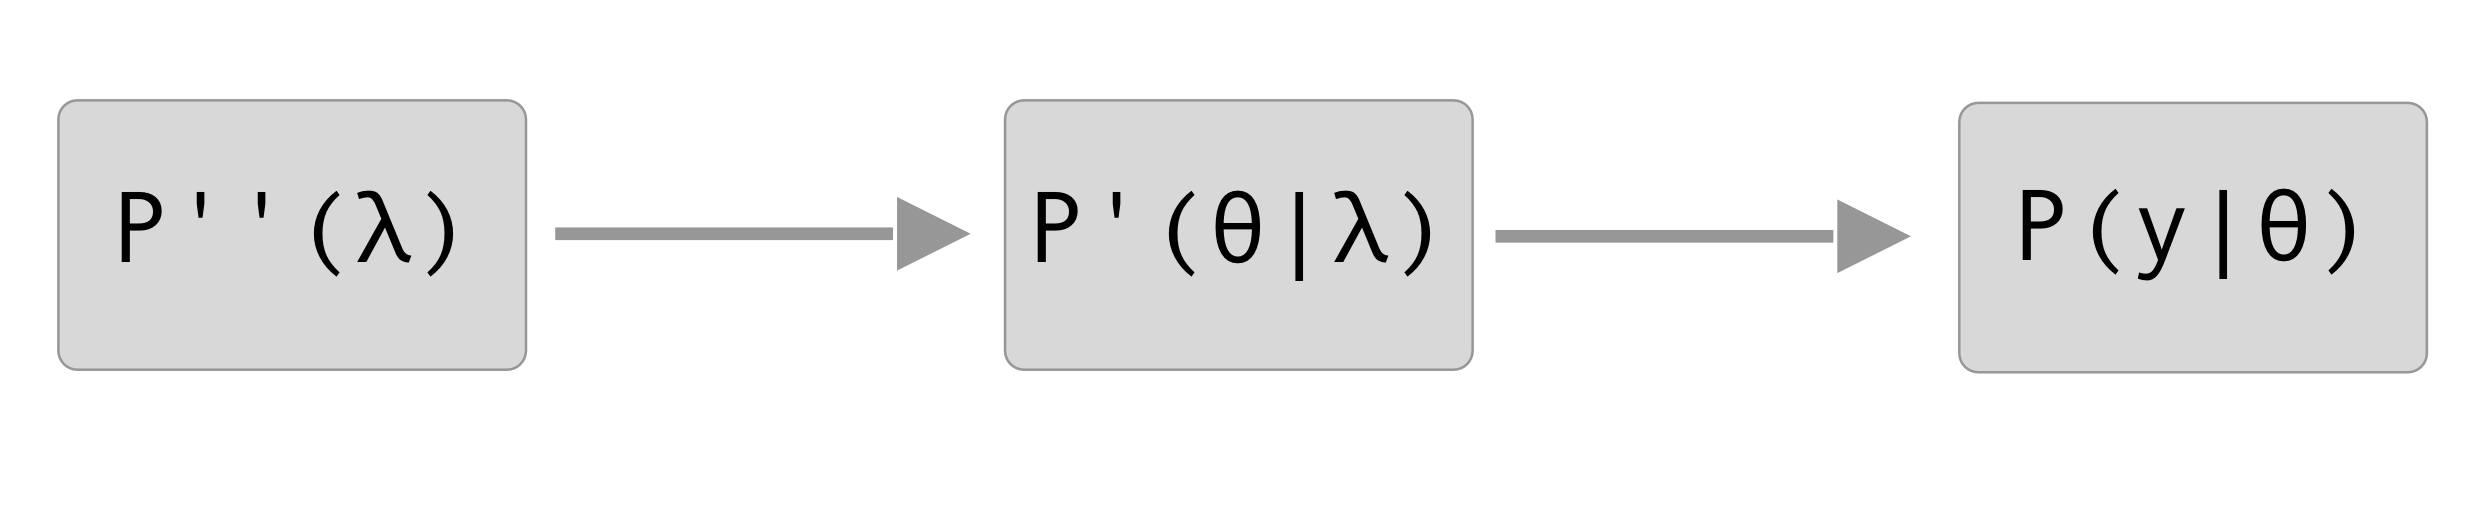
\includegraphics[width=0.5\linewidth]{images/hierarchical_relation.png}
\end{figure}

Where $P''$ is the hyperprior of the hyperparameter $\lambda$, and $P'$ is the prior of the parameter $\theta$.

\subsubsection{Parameters specification}\label{hierarchical_model}

For the purpose of this research, we will use the following model specification to estimate mortality probabilities:

\begin{equation}
    \begin{cases}
     y_{i,t+1} \sim Bernoulli(p=S(\sum_{j=1}^{k}\beta_{i,j} x_{i,j,t}))  \\
 \beta_{i,j} \sim Normal(mu=\lambda_j, std=1) \\
\lambda_j \sim Normal(mu=0, std=1) \\
    \end{cases}
\end{equation}

with $S(x)$ equal to:
\begin{equation}
     S(x) = \frac{1}{1+e^{-x}}
\end{equation}

Note that $ y_{i,t+1} $ refers to an observation of individual $i$ at time $t+1$, $\beta_{i,j}$ is the coefficient for individual $i$ and for the regressor $j$, with $j = 1,..., K$ and $\lambda_j$ is the hyperparameter of the prior. 
Each observation is treated as a Bernoulli random variable (r.v.) which is equal to:

\begin{equation}
    \begin{cases}
    1 = \text{dead} \;\; \; \text{with probability} \;\;\; p\\
    0 = \text{alive}\;\; \; \text{with probability}\;\;\; 1-p\\
    \end{cases}
\end{equation}


The parameter $p$ of the Bernoulli r.v. is set to be equal to the Sigmoid value of the sum of the individual's regressors at time $t$ times their respective estimated beta parameters.
This approach is similarly to a logistic regression.\\

To achieve information sharing and thus partial pooling between individuals, we model every individual's beta coefficient as a Normal distribution centred on a common, zero-centred normal hyperprior distribution.\\ In this way individual coefficients that would have otherwise been estimated to be very far apart will be pulled together by the underlying hyperprior and will contribute to a common knowledge about the distribution of all the other individuals' coefficients.\\
The concept of common location hyperprior can also be represented visually:\\

\begin{figure}[H]
\centering \textbf{Information sharing through a common location hyperprior} \par\medskip 
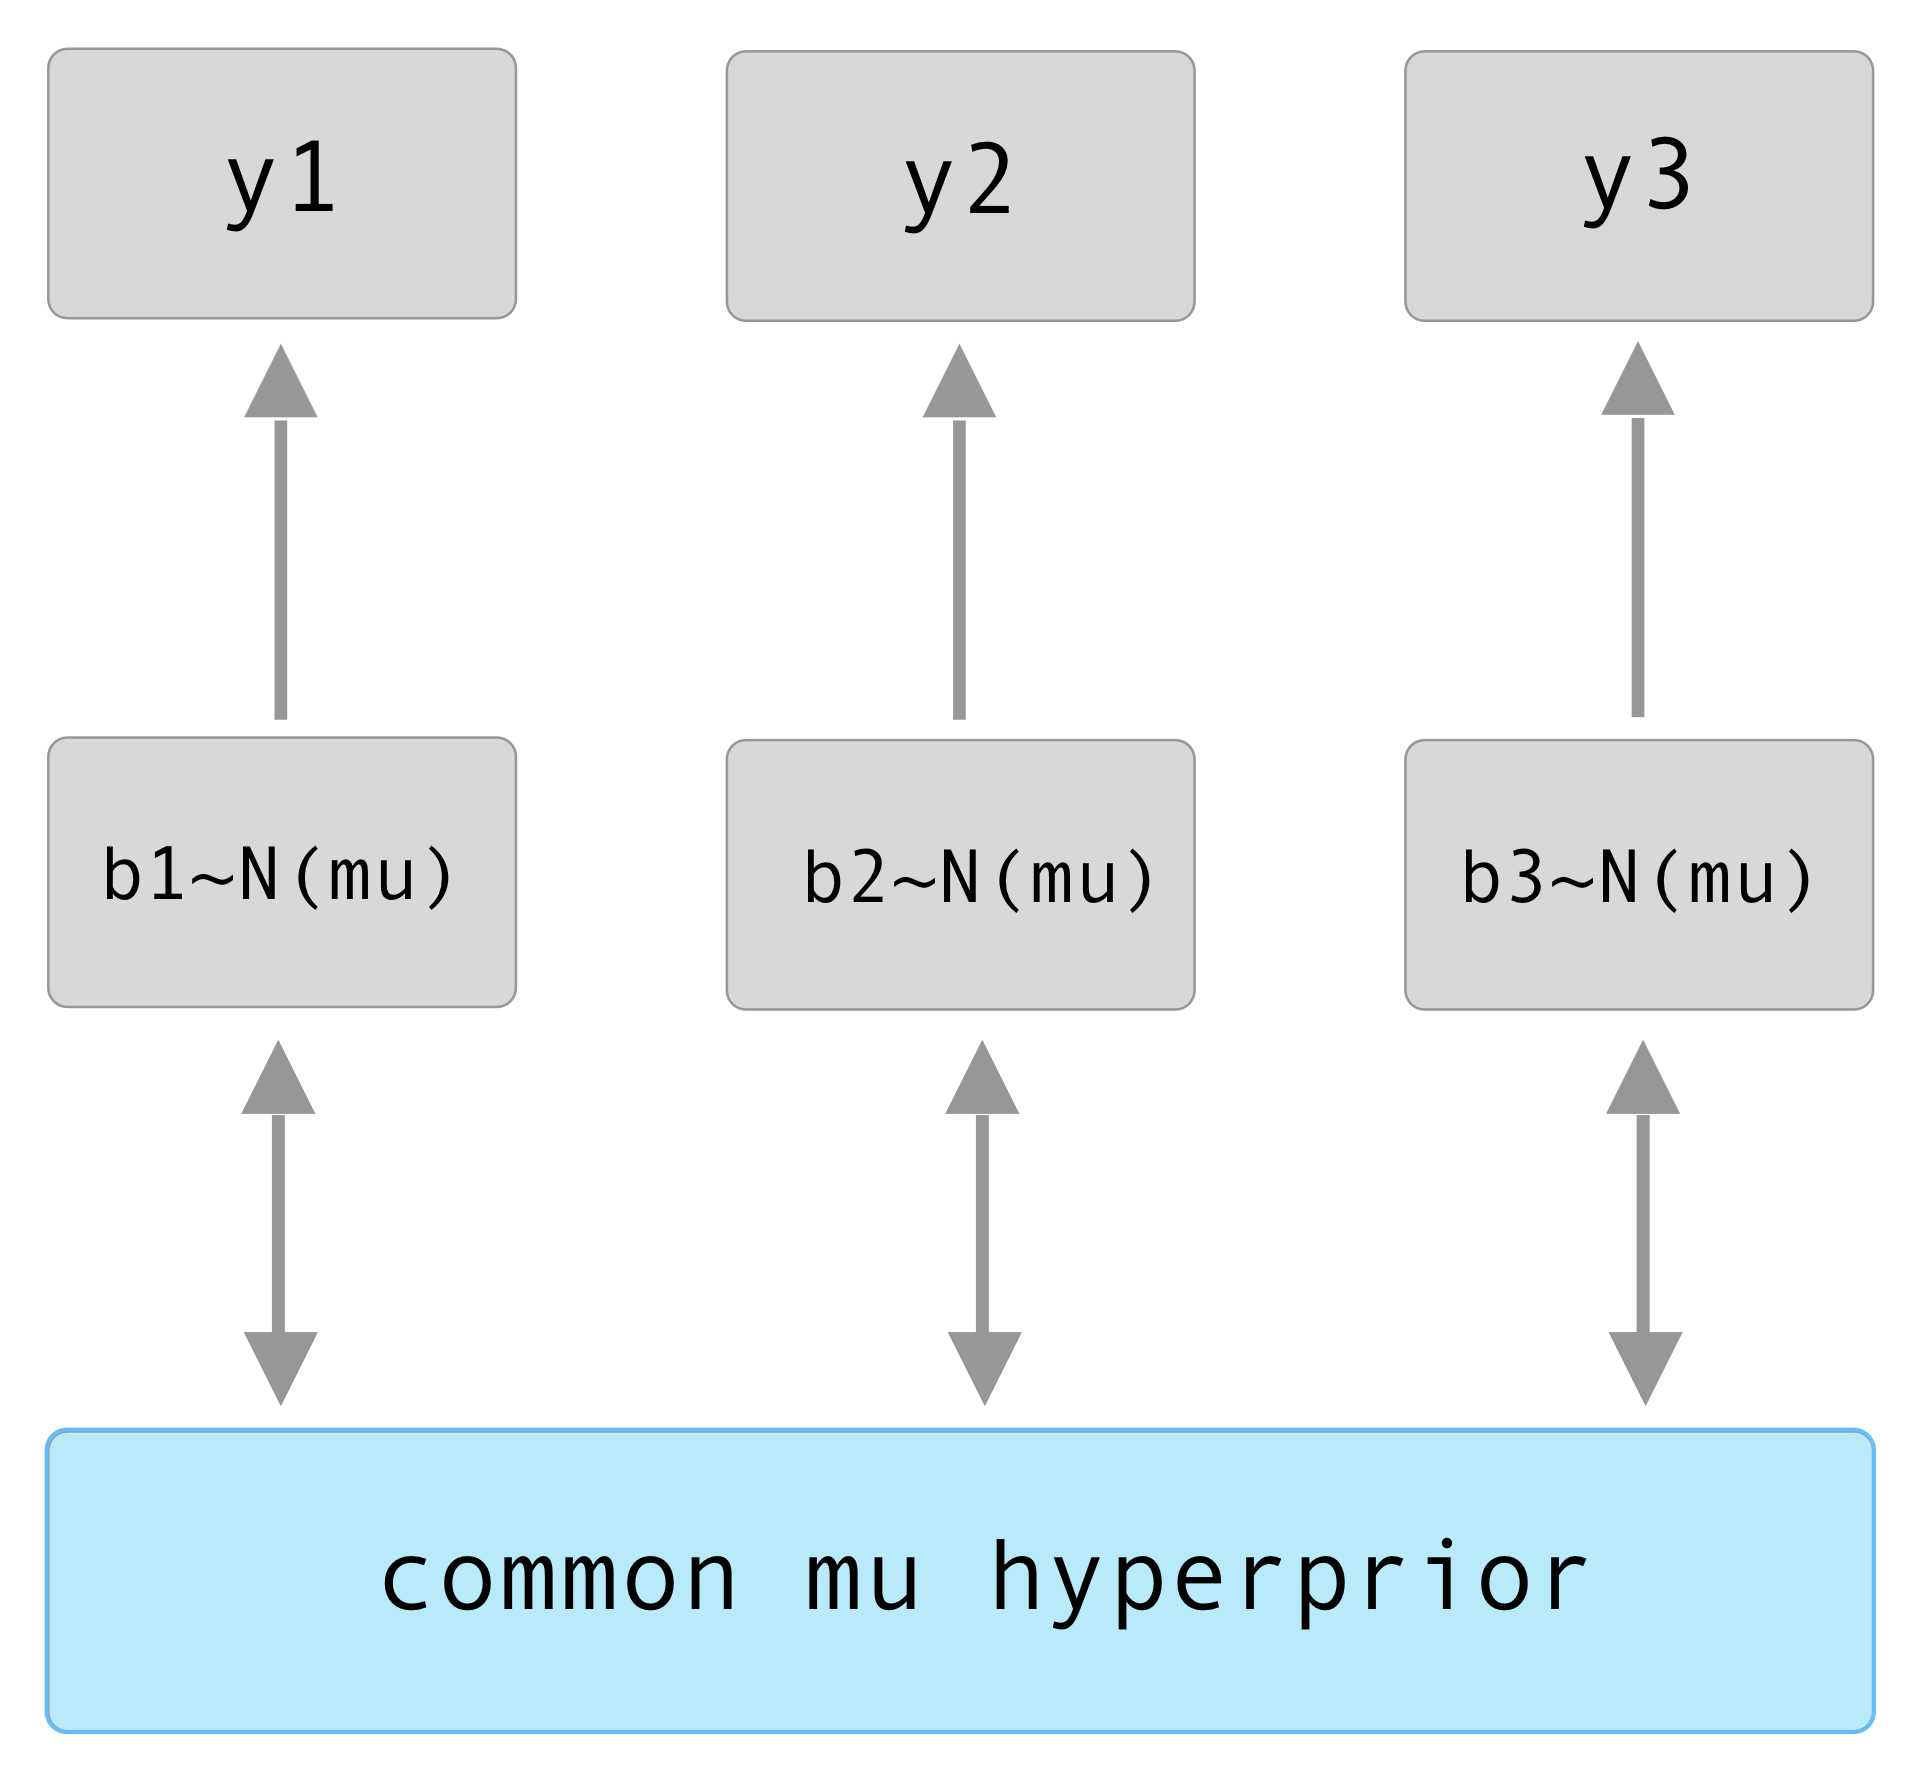
\includegraphics[width=0.4\linewidth]{images/information_sharing.png}
\end{figure}

\subsubsection{Model implementation and sampling} \label{sampling_method}

To compute the posterior distribution of our parameters given our observations, we can reformulate (1.28) by applying the rule of conditional probability: 

\begin{equation}\label{model_impl}
P(\bm{\theta} \mid \bm{y}) = \frac{P(\bm{y} \mid \bm{\theta}) P(\bm{\theta})}{P(\bm{y})}.
\end{equation}

The numerator of \ref{model_impl} is composed of $P(\bm{y} \; | \; \bm{\theta})$, i.e. the likelihood function (which represents the probability of observing our data given the parameters), and of $P(\bm{\theta})$, i.e. the prior we assumed. This first two components are quite easy to determine since the former is observed while the latter is set by the analyst. Conversely, the denominator, $P(\bm{y})$, i.e. the marginal probability of the data (which in this case serves as normalising constant) is instead less straightforward to compute.

In fact, to compute $P(\bm{y})$ we need to integrate over the whole parametric space: $$\int_{\Theta}P(y,\theta)\; d\theta$$ 
and this is often unfeasible to do analytically (especially in a hierarchical model). A solution for this problem is to use sampling algorithms of the Montecarlo Markov Chain family (in short MCMC) to achieve proposal distributions for the posterior.\\





\end{document}